\chapwithtoc{Introduction}
\label{chap:intro}

Ray tracing is a powerful image synthesis technique used in 3D computer graphics, capable of simulating optical effects, such as reflection, refraction, and scattering, with a high degree of visual realism. For this reason, it offers a variety of applications. It is used in the entertainment industry, for product design, visual prototyping, and for creating visualizations in scientific research \cite [91-128]{peddie2019ray}. Reasons for the popularity of ray tracing algorithms are the physical plausibility of its generated images as well as their simplicity and "elegance". 

The origins of ray tracing can be traced back as far as 1968. At that time, a method was invented to shade wire-framed solids by shooting random light rays from virtual light sources to the scene geometry and, if an intersection would be found, placing a symbol at the intersection point \cite{appel1968some}. If enough rays were generated, there would be a high concentration of these symbols at regions with high light intensity, which would approximate physical realism. A decade later, an elaboration of this idea to a shading model that takes global information into account for calculating light intensities  \cite{whitted1979improved}, would revolutionize the computer graphics field.

\begin{figure} \label{fig:whitted_result}
	\centering
	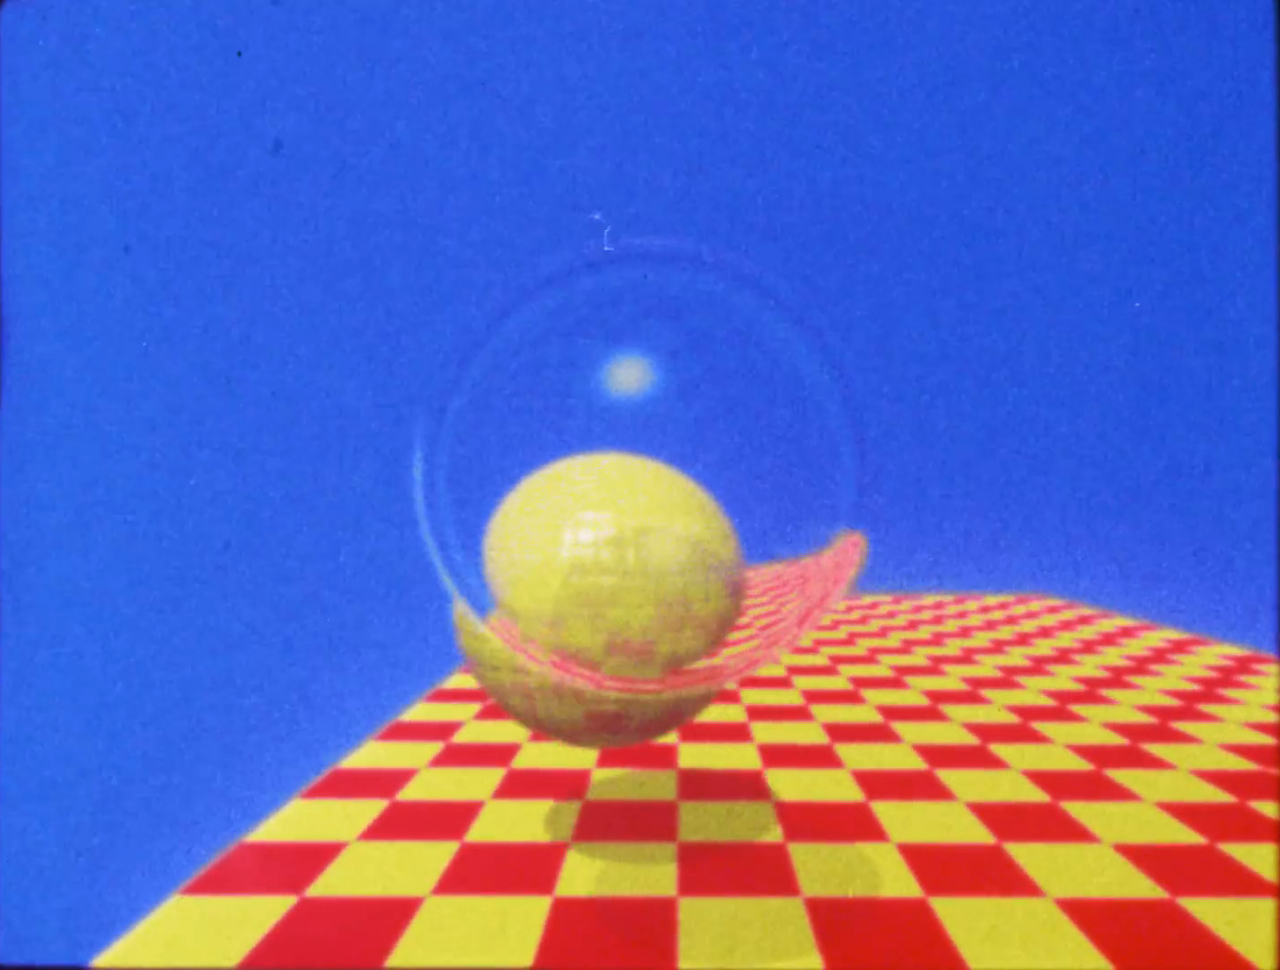
\includegraphics[width=.7\linewidth]{img/0 introduction/whitted_}
	\caption{A frame of an animation \cite{raytracingvideo} form \cite {whitted1979improved}, demonstrating recursive ray tracing, featuring a glass sphere circulating a second defuse sphere. Both are casting shadows on a diffuse checkerboard-like ground.}
	\label{fig:g}
\end{figure}

The calculation of intersection points between cast rays and scene geometry is a crucial part of ray tracing. How these points are calculated depends on the representation of geometric primitives in the scene. Primitives can be represented analytically or approximated by polygon meshes. Another possibility is the representation of a shape as a \emph{Constructive Solid Geometry (CSG)}. CSG is a hierarchical ordering of a set of primitive shapes to which Boolean set operations have been applied to. This form of representation enjoys popularity in e.g. Computer-aided geometric design.

Over the years, novel ray tracing algorithms were developed to increase the physical correctness of rendered images. However, ray tracing remains to this day a computationally demanding task. Much research was (and still is) devoted to accelerating the ray tracing procedure to compensate for its computational expense. Therefore, a wide range of researches focus on accelerating ray tracing algorithms to get better performances. Additionally, ray tracing is by nature is "embarrassingly parallel", meaning it is well suited for parallel processing by automatic vectorization. As Moore’s law predicted, the computational power in CPUs gradually increased. Nowadays, modern computers admit an integrated circuit with multiple cores on which the workload of ray tracing algorithms can be distributed. While ray tracing was considered impractical when it was pioneered, it has now become more accessible thanks to the increase of CPU power and specialized hardware.

Despite this, exploiting the computational power of modern processors to their full potential for ray tracing remains challenging. This particular reason served as the motivation for developing the award-winning (\cite{embreeAward}), open-source framework \emph{Embree} \cite{wald2014embree}. Embree offers a set of ray tracing kernels that maximize the compute capabilities of modern x86 CPU architectures.

One of the design goals behind Embree is to provide an easy integration of the framework into existing professional ray tracing environments to achieve high performance when ray tracing virtual scenes with high geometrical complexity.


\section*{Thesis subject and motivation}
The goal of this thesis is a successful integration of the Embree framework into the predictive rendering framework \emph{The Advanced Rendering Toolkit}, to facilitate the acceleration of ray tracing for constructive solid geometry.
The Advanced Rendering Toolkit will be referred to with its abbreviation \emph{ART} throughout this thesis. 

ART offers innovative features, such as efficient spectral rendering (by implementing the "Hero Wavelength Spectral Sampling" technique \cite{wilkie2014hero}), proper handling of bi-spectral materials (e.g., fluorescent surfaces) \cite{mojzik2018handling} and a physically plausible sky dome lighting model \cite{wilkie2013predicting}. Until the release of Mitsuba 2 \cite{nimier2019mitsuba}, ART was, to our best knowledge, the only rendering system that would support rendering polarization effects, and remains the sole open source rendering system to support bi-spectral reflectances. These features make ART an interesting environment for computer graphics researchers interested in the field of Predictive Rendering.

To ensure this features, ART relies on its proprietary internal data structures that diverge to a significant degree from those present in other popular rendering systems (e.g., PBRT \cite{pharr2016physically} or Mitsuba 2). Therefore, Embree's integration into ART is a non-trivial task, although Embree was developed with the intention of it being "used in existing renderers with minimal programmer effort" \cite[1]{wald2014embree}. Furthermore, Embree unfortunately does not directly support rendering CSG.

If a successful integration of Embree into ART could be achieved, a complex image synthesis system with unique predictive rendering features would be adapted to the industry standard of ray tracing. 

\section*{Thesis outline}

This thesis is structured as follows:

\begin{itemize}
	\setlength\itemsep{0.05em}
	
	\item \textbf{Chapter \ref{chap:fundamentals}} provides fundamental background information, including a brief introduction to the ray tracing technique, explanations of the most common ray acceleration structures, and a brief overview of the functionality of the Embree framework.
	
	\item \textbf{Chapter \ref{chap:technical_overview}} provides a description of Embree can be used for ray tracing and a brief introduction to ART, in which Embree will be integrated into.
	
	\item \textbf{Chapter \ref{chap:integration}} is dedicated to the description of our approach on the integration of Embree into ART, as well as the implementation of the CSG operations with Embree.
	
	\item \textbf{Chapter \ref{chap:results}} shows the results obtained by testing our implementation on various virtual scenes.
	
	\item Lastly, \textbf{Appendix \ref{sec:embree_app}} provides a user guide for compiling ART with Embree support.
	
\end{itemize}
